\documentclass[11pt,a4paper]{report}
\usepackage[textwidth=37em,vmargin=30mm]{geometry}
\usepackage{calc,xunicode,amsmath,amssymb,paralist,enumitem,tabu,booktabs,datetime2,xeCJK,xeCJKfntef,listings}
\usepackage{tocloft,fancyhdr,tcolorbox,xcolor,graphicx,eso-pic,xltxtra,xelatexemoji}

\newcommand{\envyear}[0]{2025}
\newcommand{\envdatestr}[0]{2025-01-28}
\newcommand{\envfinaldir}[0]{webdb/2025/20250128/final}

\usepackage[hidelinks]{hyperref}
\hypersetup{
    colorlinks=false,
    pdfpagemode=FullScreen,
    pdftitle={Web Digest - \envdatestr}
}

\setlength{\cftbeforechapskip}{10pt}
\renewcommand{\cftchapfont}{\rmfamily\bfseries\large\raggedright}
\setlength{\cftbeforesecskip}{2pt}
\renewcommand{\cftsecfont}{\sffamily\small\raggedright}

\setdefaultleftmargin{2em}{2em}{1em}{1em}{1em}{1em}

\usepackage{xeCJK,xeCJKfntef}
\xeCJKsetup{PunctStyle=plain,RubberPunctSkip=false,CJKglue=\strut\hskip 0pt plus 0.1em minus 0.05em,CJKecglue=\strut\hskip 0.22em plus 0.2em}
\XeTeXlinebreaklocale "zh"
\XeTeXlinebreakskip = 0pt


\setmainfont{Brygada 1918}
\setromanfont{Brygada 1918}
\setsansfont{IBM Plex Sans}
\setmonofont{JetBrains Mono NL}
\setCJKmainfont{Noto Serif CJK SC}
\setCJKromanfont{Noto Serif CJK SC}
\setCJKsansfont{Noto Sans CJK SC}
\setCJKmonofont{Noto Sans CJK SC}

\setlength{\parindent}{0pt}
\setlength{\parskip}{8pt}
\linespread{1.15}

\lstset{
	basicstyle=\ttfamily\footnotesize,
	numbersep=5pt,
	backgroundcolor=\color{black!5},
	showspaces=false,
	showstringspaces=false,
	showtabs=false,
	tabsize=2,
	captionpos=b,
	breaklines=true,
	breakatwhitespace=true,
	breakautoindent=true,
	linewidth=\textwidth
}






\newcommand{\coverpic}[2]{
    % argv: itemurl, authorname
    Cover photo by #2~~(\href{#1}{#1})
}
\newcommand{\makeheader}[0]{
    \begin{titlepage}
        % \newgeometry{hmargin=15mm,tmargin=21mm,bmargin=12mm}
        \begin{center}
            
            \rmfamily\scshape
            \fontspec{BaskervilleF}
            \fontspec{Old Standard}
            \fontsize{59pt}{70pt}\selectfont
            WEB\hfill DIGEST
            
            \vfill
            % \vskip 30pt
            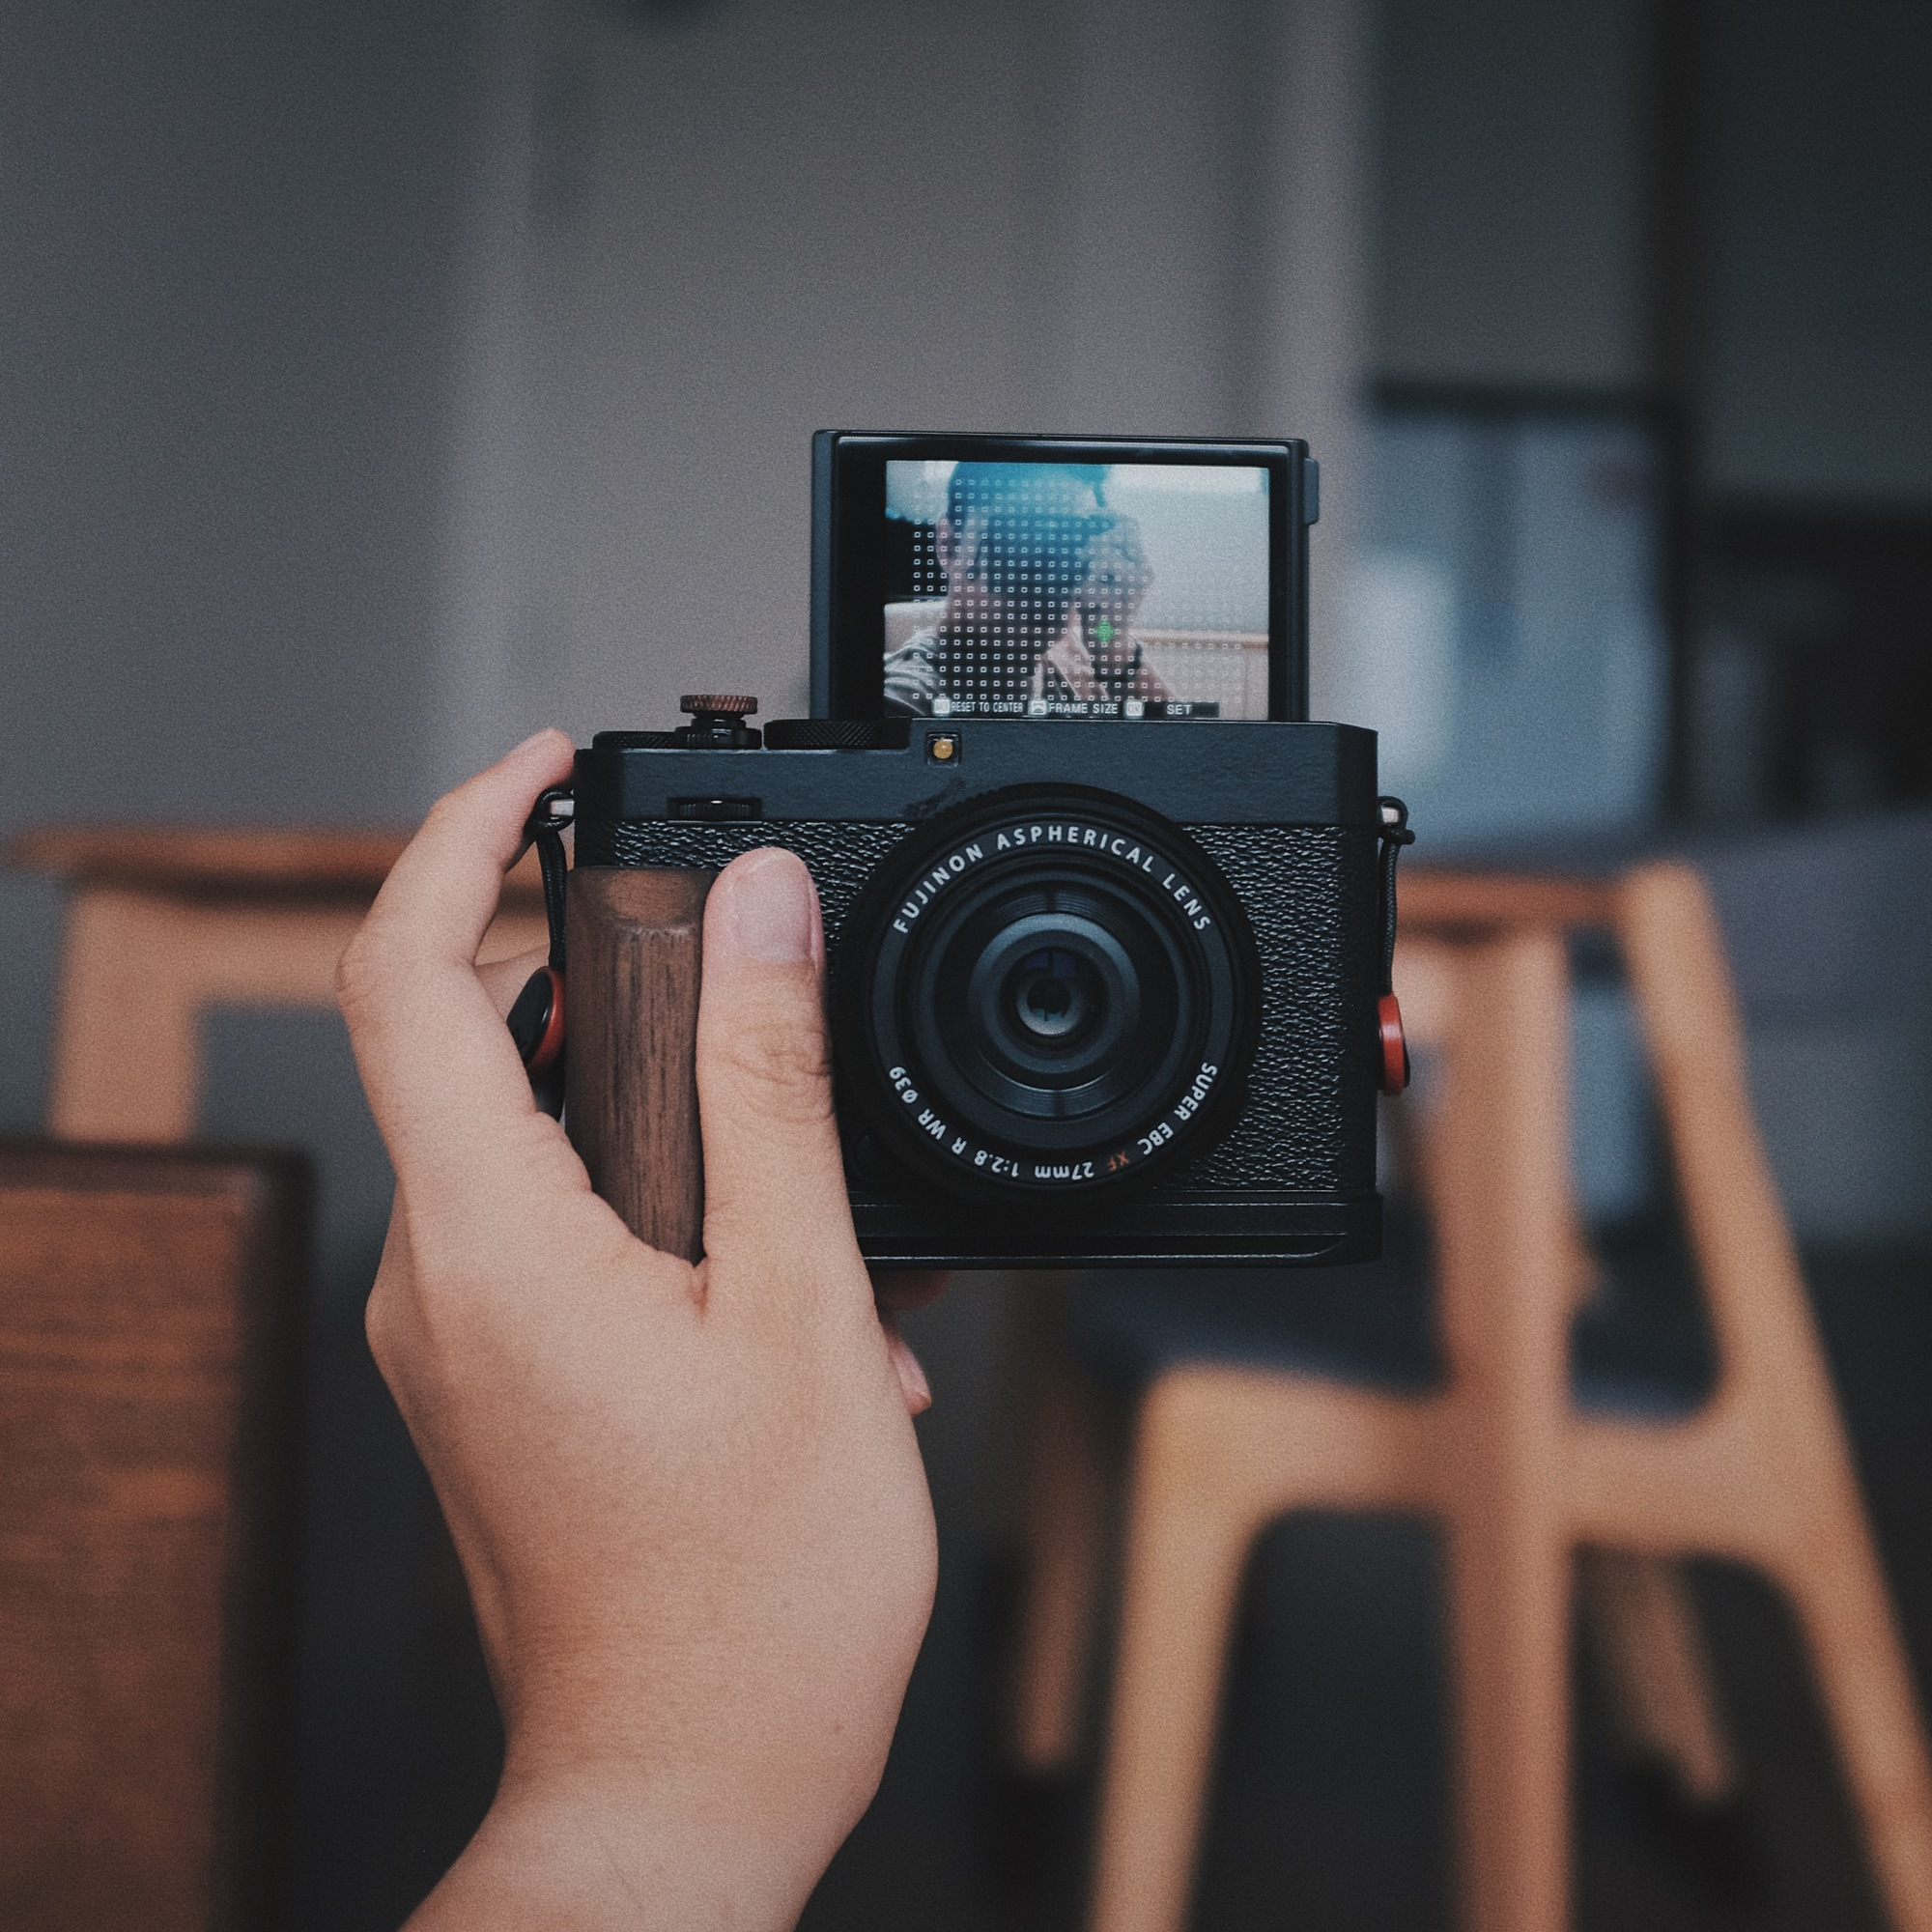
\includegraphics[width=\linewidth]{\envfinaldir/coverpic-prod.jpg}\par
            % \vskip 30pt
            \vfill

            \normalsize\rmfamily\scshape
            \copyright{} The Web Digest Project \hfill\large \envdatestr
        \end{center}
    \end{titlepage}
    % \restoregeometry
}
\newcommand{\simplehref}[1]{%
    \textcolor{blue!80!green}{\href{#1}{#1}}%
}
\renewcommand{\contentsname}{\center\Huge\sffamily\bfseries Contents\par\vskip 20pt}
\newcounter{ipartcounter}
\setcounter{ipartcounter}{0}
\newcommand{\ipart}[1]{
    % \vskip 20pt
    \clearpage
    \stepcounter{ipartcounter}
    \phantomsection
    \addcontentsline{toc}{chapter}{#1}
    % \begin{center}
    %     \Huge
    %     \sffamily\bfseries
    %     #1
    % \end{center}
    % \vskip 20pt plus 7pt
}
\newcounter{ichaptercounter}
\setcounter{ichaptercounter}{0}
\newcommand{\ichapter}[1]{
    % \vskip 20pt
    \clearpage
    \stepcounter{ichaptercounter}
    \phantomsection
    \addcontentsline{toc}{section}{\numberline{\arabic{ichaptercounter}}#1}
    \begin{center}
        \Huge
        \sffamily\bfseries
        #1
    \end{center}
    \vskip 20pt plus 7pt
}
\newcommand{\entrytitlefont}[1]{\subsection*{\raggedright\Large\sffamily\bfseries#1}}
\newcommand{\entryitemGeneric}[2]{
    % argv: title, url
    \parbox{\linewidth}{
        \entrytitlefont{#1}\par\vskip 5pt
        \footnotesize\ttfamily\mdseries
        \simplehref{#2}
    }\vskip 11pt plus 11pt minus 1pt
}
\newcommand{\entryitemGithub}[3]{
    % argv: title, url, desc
    \parbox{\linewidth}{
        \entrytitlefont{#1}\par\vskip 5pt
        \footnotesize\ttfamily\mdseries
        \simplehref{#2}\par\vskip 5pt
        \small\rmfamily\mdseries#3
    }\vskip 11pt plus 11pt minus 1pt
}
\newcommand{\entryitemAp}[3]{
    % argv: title, url, desc
    \parbox{\linewidth}{
        \entrytitlefont{#1}\par\vskip 5pt
        \footnotesize\ttfamily\mdseries
        \simplehref{#2}\par\vskip 5pt
        \small\rmfamily\mdseries#3
    }\vskip 11pt plus 11pt minus 1pt
}
\newcommand{\entryitemHackernews}[3]{
    % argv: title, hnurl, rawurl
    % \parbox{\linewidth}{
    %     \entrytitlefont{#1}\par\vskip 5pt
    %     \footnotesize\ttfamily\mdseries
    %     \simplehref{#3}\par
    %     \textcolor{black!50}{\href{#2}{#2}}
    % }\vskip 11pt plus 11pt minus 1pt
    \begin{minipage}{\linewidth}
            \entrytitlefont{#1}\par\vskip 5pt
            \footnotesize\ttfamily\mdseries
            \simplehref{#3}\par
            \textcolor{black!50}{\href{#2}{#2}}
    \end{minipage}\par\vskip 11pt plus 11pt minus 1pt
}







\begin{document}

\makeheader

\tableofcontents\clearpage




\ipart{Developers}
\ichapter{Hacker News}
\entryitemTwoLinks{I trusted an LLM, now I'm on day 4 of an afternoon project}{https://news.ycombinator.com/item?id=42845933}{https://nemo.foo/blog/day-4-of-an-afternoon-project}

\entryitemTwoLinks{Nvidia sheds almost \$600B in market cap, biggest one-day loss in US history}{https://news.ycombinator.com/item?id=42845681}{https://www.cnbc.com/2025/01/27/nvidia-sheds-almost-600-billion-in-market-cap-biggest-drop-ever.html}

\entryitemTwoLinks{The Illustrated DeepSeek-R1}{https://news.ycombinator.com/item?id=42845488}{https://newsletter.languagemodels.co/p/the-illustrated-deepseek-r1}

\entryitemTwoLinks{Go 1.24's go tool is one of the best additions to the ecosystem in years}{https://news.ycombinator.com/item?id=42845323}{https://www.jvt.me/posts/2025/01/27/go-tools-124/}

\entryitemTwoLinks{We're bringing Pebble back}{https://news.ycombinator.com/item?id=42845091}{https://repebble.com/}

\entryitemTwoLinks{Google open-sources the Pebble OS}{https://news.ycombinator.com/item?id=42845070}{https://opensource.googleblog.com/2025/01/see-code-that-powered-pebble-smartwatches.html}

\entryitemTwoLinks{The future of Rebble}{https://news.ycombinator.com/item?id=42845017}{https://rebble.io/2025/01/27/the-future-of-rebble.html}

\entryitemTwoLinks{The Alpha Myth: How captive wolves led us astray}{https://news.ycombinator.com/item?id=42844619}{https://anthonydavidadams.substack.com/p/the-alpha-myth-how-captive-wolves}

\entryitemTwoLinks{The Taylorator – All Your Frequencies Are Belong to Us}{https://news.ycombinator.com/item?id=42843623}{https://www.scd31.com/posts/taylorator}

\entryitemTwoLinks{DeepSeek releases Janus Pro, a text-to-image generator [pdf]}{https://news.ycombinator.com/item?id=42843131}{https://github.com/deepseek-ai/Janus/blob/main/janus\_pro\_tech\_report.pdf}

\entryitemTwoLinks{Operation Leg – a pilot unlike any other (2020)}{https://news.ycombinator.com/item?id=42842257}{https://www.rafbf.org/news-and-stories/raf-history/operation-leg-pilot-unlike-any-other}

\entryitemTwoLinks{My failed attempt to shrink all NPM packages by 5\%}{https://news.ycombinator.com/item?id=42840548}{https://evanhahn.com/my-failed-attempt-to-shrink-all-npm-packages-by-5-percent/}

\entryitemTwoLinks{Oliver Heaviside and the theory of transmission lines (2021)}{https://news.ycombinator.com/item?id=42840352}{https://www.pa3fwm.nl/technotes/tn28-heaviside-transmission-lines.html}

\entryitemTwoLinks{Nvidia, ASML plunge as DeepSeek triggers tech stock selloff}{https://news.ycombinator.com/item?id=42839650}{https://finance.yahoo.com/news/asml-sinks-china-ai-startup-081823609.html}

\entryitemTwoLinks{Facebook ban on discussing Linux?}{https://news.ycombinator.com/item?id=42839502}{https://distrowatch.com/weekly-mobile.php?issue=20250127\#sitenews}

\entryitemTwoLinks{SiFive's P550 Microarchitecture}{https://news.ycombinator.com/item?id=42839501}{https://chipsandcheese.com/p/inside-sifives-p550-microarchitecture}

\entryitemTwoLinks{Sweden Seizes Ship Suspected of Baltic Sea 'Sabotage'}{https://news.ycombinator.com/item?id=42839348}{https://www.barrons.com/news/sweden-says-has-seized-ship-suspected-of-baltic-sea-sabotage-13ff82f2}

\entryitemTwoLinks{Show HN: I Made an iOS Podcast Player with Racket}{https://news.ycombinator.com/item?id=42838875}{https://defn.io/2024/11/16/podcatcher/}

\entryitemTwoLinks{One in four 2020 Tesla Model 3 failed the Danish periodic inspection in 2024}{https://news.ycombinator.com/item?id=42838855}{https://fdm.dk/nyheder/bilist/2025-01-populaer-tesla-model-dumper-med-et-brag-til-syn}

\entryitemTwoLinks{A layoff fundamentally changed how I perceive work}{https://news.ycombinator.com/item?id=42838700}{https://mertbulan.com/2025/01/26/once-you-are-laid-off-you-will-never-be-the-same-again/}\ichapter{Phoronix}
\entryitemGeneric{\hskip 0pt{}Llama.cpp AI Performance With The GeForce RTX 5090}{https://www.phoronix.com/review/nvidia-rtx5090-llama-cpp}

\entryitemGeneric{\hskip 0pt{}AMD ZenDNN 5.0 Software For AI Delivers "400\% Performance Uplift"}{https://www.phoronix.com/news/AMD-ZenDNN-5.0-400p-Performance}

\entryitemGeneric{\hskip 0pt{}Hyprland 0.47 Wayland Compositor Delivers Experimental HDR, GPU Hotplugging}{https://www.phoronix.com/news/Hyprland-0.47-Released}

\entryitemGeneric{\hskip 0pt{}GNOME Triple Buffering Now Works With Direct Scanout \& VRR}{https://www.phoronix.com/news/GNOME-Triple-Buffering-Direct}

\entryitemGeneric{\hskip 0pt{}Laptop Improvements \& More AMD Driver Features Merged For Linux 6.14}{https://www.phoronix.com/news/Linux-6.14-x86-Platform-Drivers}

\entryitemGeneric{\hskip 0pt{}NAMD Molecular Dynamics Performance Improves Well With NVIDIA Blackwell / RTX 5090}{https://www.phoronix.com/news/NAMD-NVIDIA-GeForce-RTX-5090}

\entryitemGeneric{\hskip 0pt{}Reduced SquashFS Memory Use With The Linux 6.14 Kernel, More NILFS2 Fixes}{https://www.phoronix.com/news/Linux-6.14-Non-MM}

\entryitemGeneric{\hskip 0pt{}Desktop Motherboards Continue Playing Catch-Up For Linux Monitoring Support}{https://www.phoronix.com/news/Linux-6.14-HWMON}

\entryitemGeneric{\hskip 0pt{}Microsoft Announces Open-Source DocumentDB NoSQL Database}{https://www.phoronix.com/news/Microsoft-OpenSource-DocumentDB}\ichapter{Dribbble}
\entryitemGeneric{\hskip 0pt{}Speed Test App Ui Design}{https://dribbble.com/shots/25535763-Speed-Test-App-Ui-Design}

\entryitemGeneric{\hskip 0pt{}Dyna - Logo Design}{https://dribbble.com/shots/25525428-Dyna-Logo-Design}

\entryitemGeneric{\hskip 0pt{}B}{https://dribbble.com/shots/25524895-B}

\entryitemGeneric{\hskip 0pt{}Godzilla Logo}{https://dribbble.com/shots/25525727-Godzilla-Logo}

\entryitemGeneric{\hskip 0pt{}Peregrine Engineering®}{https://dribbble.com/shots/25527465-Peregrine-Engineering}

\entryitemGeneric{\hskip 0pt{}VCC Unused Logo Concept - V4}{https://dribbble.com/shots/25525024-VCC-Unused-Logo-Concept-V4}

\entryitemGeneric{\hskip 0pt{}M for Mountain Logo Design (Unused for Sale)}{https://dribbble.com/shots/25524897-M-for-Mountain-Logo-Design-Unused-for-Sale}

\entryitemGeneric{\hskip 0pt{}Tattooed Devil Horns}{https://dribbble.com/shots/25520911-Tattooed-Devil-Horns}

\entryitemGeneric{\hskip 0pt{}Fitness and Step Count app UI Design}{https://dribbble.com/shots/25518949-Fitness-and-Step-Count-app-UI-Design}

\entryitemGeneric{\hskip 0pt{}Carbon Solutions B2B Dashboard Design}{https://dribbble.com/shots/25506638-Carbon-Solutions-B2B-Dashboard-Design}

\entryitemGeneric{\hskip 0pt{}Goose Gym}{https://dribbble.com/shots/25515121-Goose-Gym}

\entryitemGeneric{\hskip 0pt{}Rapid Rabbit Logo}{https://dribbble.com/shots/25516738-Rapid-Rabbit-Logo}

\entryitemGeneric{\hskip 0pt{}LLM GPU Manager}{https://dribbble.com/shots/25513811-LLM-GPU-Manager}

\entryitemGeneric{\hskip 0pt{}HappyDev - Logo Design / Branding}{https://dribbble.com/shots/25514894-HappyDev-Logo-Design-Branding}

\entryitemGeneric{\hskip 0pt{}Product design - icons set}{https://dribbble.com/shots/25516253-Product-design-icons-set}

\entryitemGeneric{\hskip 0pt{}VCC Unused Logo Design Concept}{https://dribbble.com/shots/25511334-VCC-Unused-Logo-Design-Concept}

\entryitemGeneric{\hskip 0pt{}The Toucan}{https://dribbble.com/shots/25515890-The-Toucan}

\entryitemGeneric{\hskip 0pt{}Bestest Brand®}{https://dribbble.com/shots/25510300-Bestest-Brand}

\entryitemGeneric{\hskip 0pt{}QVELTY / Design \& Animation}{https://dribbble.com/shots/25507639-QVELTY-Design-Animation}

\entryitemGeneric{\hskip 0pt{}Haptic Logo Design}{https://dribbble.com/shots/25504012-Haptic-Logo-Design}

\entryitemGeneric{\hskip 0pt{}Wine Label}{https://dribbble.com/shots/25509757-Wine-Label}

\entryitemGeneric{\hskip 0pt{}Letter V + LED + Wires Logo}{https://dribbble.com/shots/25507506-Letter-V-LED-Wires-Logo}

\entryitemGeneric{\hskip 0pt{}Robin bird logo}{https://dribbble.com/shots/25509208-Robin-bird-logo}

\entryitemGeneric{\hskip 0pt{}Qore - Logo Design}{https://dribbble.com/shots/25509466-Qore-Logo-Design}


\ipart{Developers~~~~(zh-Hans)}
\ichapter{Solidot}
\entryitemGeneric{\hskip 0pt{}Onlyfans 成功背后的心理学}{https://www.solidot.org/story?sid=80440}

\entryitemGeneric{\hskip 0pt{}科学家通过黑洞合并事件验证宇宙镜像对称性}{https://www.solidot.org/story?sid=80439}

\entryitemGeneric{\hskip 0pt{}研究揭示 PM2.5 毒理学机制}{https://www.solidot.org/story?sid=80438}

\entryitemGeneric{\hskip 0pt{}DeepSeek 登顶苹果应用商店免费应用排行榜}{https://www.solidot.org/story?sid=80437}

\entryitemGeneric{\hskip 0pt{}天文学家呼吁禁止太空广告}{https://www.solidot.org/story?sid=80436}

\entryitemGeneric{\hskip 0pt{}研究发现对 AI 了解越少的人越愿意使用 AI}{https://www.solidot.org/story?sid=80435}

\entryitemGeneric{\hskip 0pt{}特斯拉拒绝将 FSD 软件转移到新车}{https://www.solidot.org/story?sid=80434}

\entryitemGeneric{\hskip 0pt{}Bitmanagement 与美国海军的反盗版诉讼再次受挫}{https://www.solidot.org/story?sid=80433}

\entryitemGeneric{\hskip 0pt{}GLP-1RA 的益处和风险}{https://www.solidot.org/story?sid=80431}

\entryitemGeneric{\hskip 0pt{}研究人员发现中欧电网用非加密无线信号控制}{https://www.solidot.org/story?sid=80430}

\entryitemGeneric{\hskip 0pt{}甲骨文等正在谈判接手 TikTok 美国业务}{https://www.solidot.org/story?sid=80428}

\entryitemGeneric{\hskip 0pt{}小鼠研究发现微塑料会堵塞大脑血液流动}{https://www.solidot.org/story?sid=80427}

\entryitemGeneric{\hskip 0pt{}ADHD 患者有更短的预期寿命}{https://www.solidot.org/story?sid=80426}

\entryitemGeneric{\hskip 0pt{}研究称电动汽车的寿命与燃油汽车相差无几}{https://www.solidot.org/story?sid=80425}

\entryitemGeneric{\hskip 0pt{}大英博物馆遭前 IT 雇员攻击而部分关闭}{https://www.solidot.org/story?sid=80424}

\entryitemGeneric{\hskip 0pt{}巴基斯坦议会通过法案全面控制社交媒体}{https://www.solidot.org/story?sid=80423}

\entryitemGeneric{\hskip 0pt{}AI 犯的错误和人类不同}{https://www.solidot.org/story?sid=80422}

\entryitemGeneric{\hskip 0pt{}数百超级富豪呼吁对其征收更高的税}{https://www.solidot.org/story?sid=80421}

\entryitemGeneric{\hskip 0pt{}Linux 6.14 加入对微软 Copilot 按键的支持}{https://www.solidot.org/story?sid=80420}

\entryitemGeneric{\hskip 0pt{}秘密后门使用``魔法封包''感染企业 VPN}{https://www.solidot.org/story?sid=80419}\ichapter{V2EX}
\entryitemGeneric{\hskip 0pt{}[问与答] 飛信為什麼會失敗?}{https://www.v2ex.com/t/1108148}

\entryitemGeneric{\hskip 0pt{}[Apple] 备忘录 Notes 内容被误删除,无法恢复}{https://www.v2ex.com/t/1108147}

\entryitemGeneric{\hskip 0pt{}[程序员] 结合 deepseek R1 模型,新的 AI Cursor 编程最佳实践!让第三方 ai 成为我们和 cursor 沟通的桥梁}{https://www.v2ex.com/t/1108146}

\entryitemGeneric{\hskip 0pt{}[问与答] Google voice 突然没了}{https://www.v2ex.com/t/1108145}

\entryitemGeneric{\hskip 0pt{}[iPad] iPad 版 Chrome 打字巨卡}{https://www.v2ex.com/t/1108143}

\entryitemGeneric{\hskip 0pt{}[分享发现] DeepSeek: ``斯普特尼克时刻''。AI 冷战?}{https://www.v2ex.com/t/1108141}

\entryitemGeneric{\hskip 0pt{}[OpenWrt] openwrt 搭建 tamspeak 只能内网访问如何解决?}{https://www.v2ex.com/t/1108140}

\entryitemGeneric{\hskip 0pt{}[问与答] 剪映的双语字幕要求会员才可以导出视频,有没有替代版本或者软件?}{https://www.v2ex.com/t/1108139}

\entryitemGeneric{\hskip 0pt{}[分享发现] deepseek 锐评 v2ex}{https://www.v2ex.com/t/1108138}

\entryitemGeneric{\hskip 0pt{}[问与答] 原生家庭,过年刚回家和家里白眼狼姐打起来了}{https://www.v2ex.com/t/1108137}

\entryitemGeneric{\hskip 0pt{}[程序员] ProxMonitor 用于监控和管理 Proxmox VE 服务器的 Android 应用}{https://www.v2ex.com/t/1108136}

\entryitemGeneric{\hskip 0pt{}[分享发现] 近期 DeepSeek 线上服务受到大规模恶意攻击,为持续提供服务,暂时限制了+86 手机号以外的注册方式,已注册用户可以正常登录,感谢理解和支持}{https://www.v2ex.com/t/1108134}

\entryitemGeneric{\hskip 0pt{}[分享发现] 极客湾对 2024 年性能手机的评测}{https://www.v2ex.com/t/1108131}

\entryitemGeneric{\hskip 0pt{}[问与答] 2025 重装 Windows 系统后如何快速安装常用软件?}{https://www.v2ex.com/t/1108130}

\entryitemGeneric{\hskip 0pt{}[职场话题] 外企简历筛选是怎么样的}{https://www.v2ex.com/t/1108129}

\entryitemGeneric{\hskip 0pt{}[生活] 碰到这种情况该怎么处理}{https://www.v2ex.com/t/1108128}

\entryitemGeneric{\hskip 0pt{}[问与答] putty 连接 Linux ,如何将 vim 模式下的文本复制到 win 的剪切板中?}{https://www.v2ex.com/t/1108126}

\entryitemGeneric{\hskip 0pt{}[Apple] 如何优雅的备份 livephoto}{https://www.v2ex.com/t/1108125}

\entryitemGeneric{\hskip 0pt{}[程序员] 群晖下 docker 容器 bridge 隔离网可以直接访问宿主机}{https://www.v2ex.com/t/1108124}

\entryitemGeneric{\hskip 0pt{}[macOS] M1 芯片 MacOS15.2 双显示器使用,第三方和系统自带的"其他"栏下的屏保——都只能在扩展显示器显示,主显示器无法显示。}{https://www.v2ex.com/t/1108123}

\entryitemGeneric{\hskip 0pt{}[程序员] 小白请教:买一个 Mac mini M4 当服务器用,合适不。}{https://www.v2ex.com/t/1108122}

\entryitemGeneric{\hskip 0pt{}[天黑以后] 20250127 午夜俱乐部}{https://www.v2ex.com/t/1108121}

\entryitemGeneric{\hskip 0pt{}[问与答] 流量分流,国外的走 SIM 卡,国内的走宽带}{https://www.v2ex.com/t/1108120}

\entryitemGeneric{\hskip 0pt{}[分享发现] 来刷短视频,看直播吧,真的很好看。}{https://www.v2ex.com/t/1108119}

\entryitemGeneric{\hskip 0pt{}[问与答] 微图坊 v2ph 有替代品吗}{https://www.v2ex.com/t/1108118}

\entryitemGeneric{\hskip 0pt{}[问与答] 为什么 xbox series 手柄会断连}{https://www.v2ex.com/t/1108117}

\entryitemGeneric{\hskip 0pt{}[问与答] 求 v 友推荐路由器!}{https://www.v2ex.com/t/1108116}

\entryitemGeneric{\hskip 0pt{}[Python] 初一的孩子想要学 Python , 有好的视频集合推荐吗, 孩子能看得懂的书也可以}{https://www.v2ex.com/t/1108115}

\entryitemGeneric{\hskip 0pt{}[分享发现] 独立开发周记 102:金蛇送福}{https://www.v2ex.com/t/1108113}

\entryitemGeneric{\hskip 0pt{}[分享发现] 大模型混战:请按照《过秦论》的风格,写一篇过``美利坚论''}{https://www.v2ex.com/t/1108112}

\entryitemGeneric{\hskip 0pt{}[OpenWrt] OpenWrt 下,静态 DHCP 分配 ipv4 的主机,能配置独立的 ipv6 的 dns 吗?}{https://www.v2ex.com/t/1108111}

\entryitemGeneric{\hskip 0pt{}[问与答] 关于新加坡 OCBC 相关讨论下}{https://www.v2ex.com/t/1108110}

\entryitemGeneric{\hskip 0pt{}[问与答] 产品设计图生成+ai 也是一个应用场景}{https://www.v2ex.com/t/1108109}

\entryitemGeneric{\hskip 0pt{}[酷工作] [珠海] 招前端开发一个。}{https://www.v2ex.com/t/1108108}

\entryitemGeneric{\hskip 0pt{}[问与答] 求问有没有支持两个或以上访客 WIFI 的路由器?}{https://www.v2ex.com/t/1108107}

\entryitemGeneric{\hskip 0pt{}[问与答] 为什么我现在路过农村看到漂亮的自建房,二层的觉得很美,三层的就觉得很普通}{https://www.v2ex.com/t/1108106}

\entryitemGeneric{\hskip 0pt{}[问与答] 过年了,你开心吗?}{https://www.v2ex.com/t/1108105}

\entryitemGeneric{\hskip 0pt{}[微信] 过年回趟家发现微信小程序上那么多垃圾商城平台}{https://www.v2ex.com/t/1108104}

\entryitemGeneric{\hskip 0pt{}[问与答] DeepSeek 有人用了没?体验怎么样?}{https://www.v2ex.com/t/1108102}

\entryitemGeneric{\hskip 0pt{}[程序员] AI 辅助编程 + Trae 体验测评 + 5000+ 字长文,介绍下对 AI 辅助变成的探索与反思}{https://www.v2ex.com/t/1108101}

\entryitemGeneric{\hskip 0pt{}[问与答] 请问树莓派做 nas 有什么好用的系统?}{https://www.v2ex.com/t/1108100}

\entryitemGeneric{\hskip 0pt{}[他他] 文明聊天,出柜交友、求职招聘、生活情调、八卦吐槽、花花草草、猫猫狗狗}{https://www.v2ex.com/t/1108099}

\entryitemGeneric{\hskip 0pt{}[分享发现] 各位小伙伴,今年辛苦了}{https://www.v2ex.com/t/1108098}

\entryitemGeneric{\hskip 0pt{}[问与答] 有推荐类似于 Mac mini 的高性价比 Linux 小主机么?}{https://www.v2ex.com/t/1108097}

\entryitemGeneric{\hskip 0pt{}[分享创造] 反思了一下维护 500 多天的开源项目}{https://www.v2ex.com/t/1108096}

\entryitemGeneric{\hskip 0pt{}[问与答] 有没有新手画房子构造图的软件呢?比较简单的}{https://www.v2ex.com/t/1108095}

\entryitemGeneric{\hskip 0pt{}[问与答] DeepSeek 是不是颠覆了以往对 GPU 的大需求?}{https://www.v2ex.com/t/1108093}

\entryitemGeneric{\hskip 0pt{}[问与答] 如何提升父母幸福感}{https://www.v2ex.com/t/1108091}

\entryitemGeneric{\hskip 0pt{}[分享创造] 做了个 1 分钟出拜年海报的 AI 小程序}{https://www.v2ex.com/t/1108089}


\ipart{Generic News}







\clearpage
\leavevmode\vfill
\footnotesize

Copyright \copyright{} 2023-2025 Neruthes and other contributors.

This document is published with CC BY-NC-ND 4.0 license.

The entries listed in this newsletter may be copyrighted by their respective creators.

This newsletter is generated by the Web Digest project.

The newsletters are also delivered via Telegram channel \CJKunderline{\href{https://t.me/webdigestchannel}{https://t.me/webdigestchannel}}.\\
RSS feed is available at \CJKunderline{\href{https://webdigest.pages.dev/rss.xml}{https://webdigest.pages.dev/rss.xml}}.

This newsletter is available in PDF at
\CJKunderline{\href{https://webdigest.pages.dev/}{https://webdigest.pages.dev/}}.

The source code being used to generate this newsletter is available at\\
\CJKunderline{\href{https://github.com/neruthes/webdigest}{https://github.com/neruthes/webdigest}}.

This newsletter is also available in
\CJKunderline{\href{http://webdigest.pages.dev/readhtml/\envyear/WebDigest-20250128.html}{HTML}} and
\CJKunderline{\href{https://github.com/neruthes/webdigest/blob/master/markdown/\envyear/WebDigest-20250128.md}{Markdown}}.


\coverpic{https://unsplash.com/photos/a-man-is-seen-through-a-circular-lens-8DL9SnGLSy4}{Dominik Mecko}


\end{document}
